
%*******************************************************
% Chapter 1
%*******************************************************

\myChapter{Implementation notes}

\begin{refsection}

It is worth summarizing few notes about implementation.


\begin{figure}
   \centering
   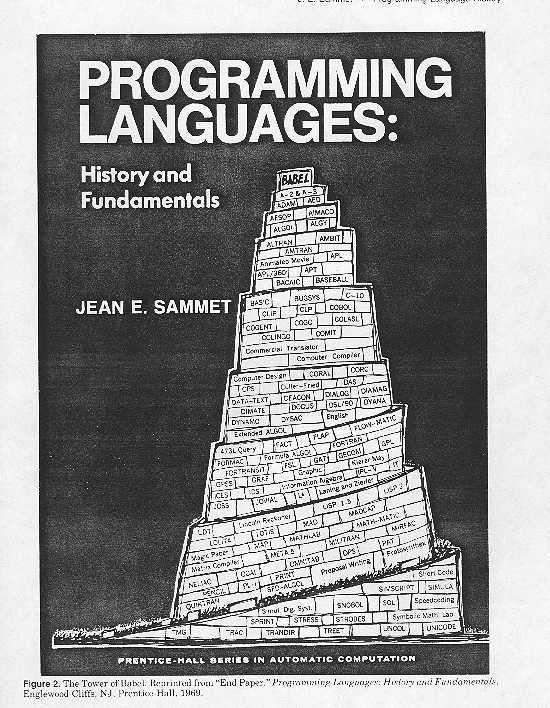
\includegraphics[width=.5\textwidth]{babel}
   \caption{The Babel's Tower of programming languages, taken from the cover of
      J. Sammet's \emph{Programming Languages: History and Fundamentals} (1969).
      Being a 1969 book, the picture misses several important additions,
      nevertheless it is still representative of the difficulty in choosing a
      suitable programming language.
   }
\end{figure}

\section{Glimpse at functional programming languages}
Functional programming languages has gained attraction over imperative ones in recent years due to
their ability to handle effortlessly and in robust way concurrency and
multithreading/multicore 
computing, making them particularly suitable to distributed frameworks. 

Historically, concurrent programming was not the original motivation for
functional programming. 
After the early functional-flavored language Lisp and  the development of APL in the
early 1960s by Iverson, functional programming was eventually formalized by
John Bakus (the father of Fortran) in his
cornerstone 1977 Turing Award Lecture 
\emph{Can Programming Be Liberated From the von Neumann Style?
   A Functional Style and its Algebra of Programs}, where he presented his FP
programming language and emphasizes how liberating a programming language from
the traditional imperative style would have lead to a programming language
closer to mathematical abstractions. 

For several years, functional programming was relegated mainly as an academic
tool. Nevertheless, several powerful functional programming languages have been
developed in the last decades. It is worth mentioning at this point:
Haskell, Erlang, OCam, Closure. 
Scala was build 

\section{Reactive paradigm}

\section{Python}   

\section{IPython  and other notebooks}   
\section{Scala}

\section{Cern ROOT for HEP}
In high-energy physics

\section{Distributed programming: Apache Spark}


\printbibliography[heading=subbibliography]
\end{refsection}
